% 2015
% Maciej Szeptuch
% II UWr

\documentclass[11pt,leqno]{article}

\usepackage[utf8]{inputenc}
\usepackage{polski}
\usepackage{a4wide}
\usepackage[cm]{fullpage}

\usepackage{multicol}
\usepackage{graphicx}
\usepackage{epstopdf}
\usepackage{amsmath,amssymb}
\usepackage{bm}
\usepackage{amsthm}

\usepackage{wrapfig}

%% Kropka po numerze paragrafu, podparagrafu, itp.
\makeatletter
    \renewcommand\@seccntformat[1]{\csname the#1\endcsname.\quad}
    \renewcommand\numberline[1]{#1.\hskip0.7em}
\makeatother

%% Numeracja wzorów
\renewcommand{\theequation}{\arabic{section}.\arabic{equation}}

%%%%%%%%%%%%%%%%%%%%%%%%%%%%%%%%%%%%%%%%%%%%%%%%%%%%%%%%%%%%%%%%%%%%%%%%%%%%%%%%

\title{Zastosowanie sieci neuronowych do generowania tekstu}
\author{Maciej Szeptuch}
\date{Wrocław, \today}

\begin{document}
\thispagestyle{empty}
\maketitle

\section{Opis}
Zastosowałem sieci neuronowe do generowania/dopełniania tekstu na podstawie podanego jako wejście prefiksu.
Znalazłem, że jednym z lepszych jeśli nie najlepszym modelem do takich zastosowań są nawracające sieci neuronowe(recurrent neural networks) - przynajmniej w teorii. \\
W praktyce sprawiają one wiele problemów, przy wykorzystaniu SGD trzeba bardzo uważać na wszystkie parametry i współczynniki podczas nauczania, ponieważ gradient potrafi w nieoczekiwanych momentach eksplodować.
W niektórych pracach jest też zastosowana metoda nazywana Hesian-Free optimization, jej główną zaletą jest to, że jest bardzo stabilna - w szczególności w porównaniu do SGD, a główną wadą to że jest nieporównywalnie wolna.
\\\\
Próbowałem wykorzystać obie metody na danych z podkorpusu milionowego NKJP, konkretnie wyciąłem z niego wszystkie zdania (ok. 45000).

\section{Dane}
\subsection{Znak po znaku}
Trochę statystyk z danych:
\begin{itemize}
    \item Liczba zdań: 45000
    \item Liczba różnych znaków: 63
    \item Długość zdań: od 23 do 551 znaków, średnio: 101 znaków
\end{itemize}
\begin{figure}[!h]
    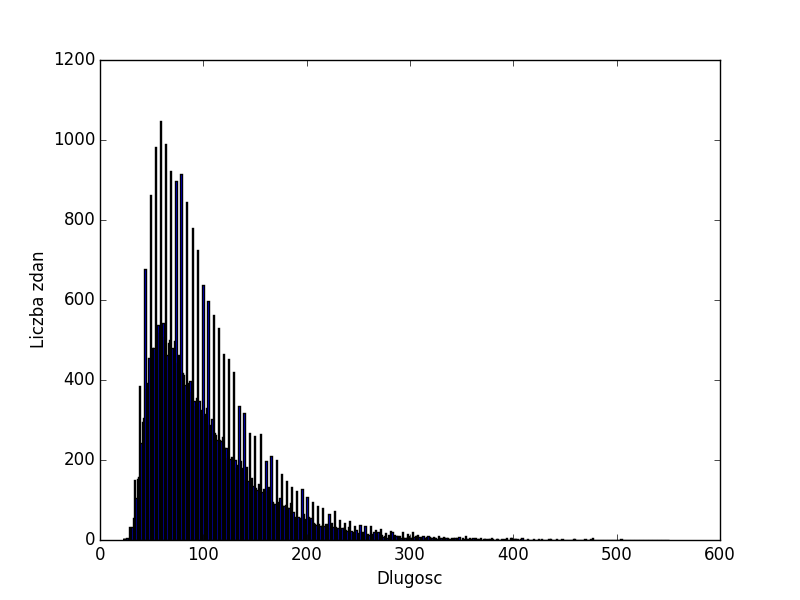
\includegraphics[width=0.5\textwidth]{pictures/char_length_distribution.png}
    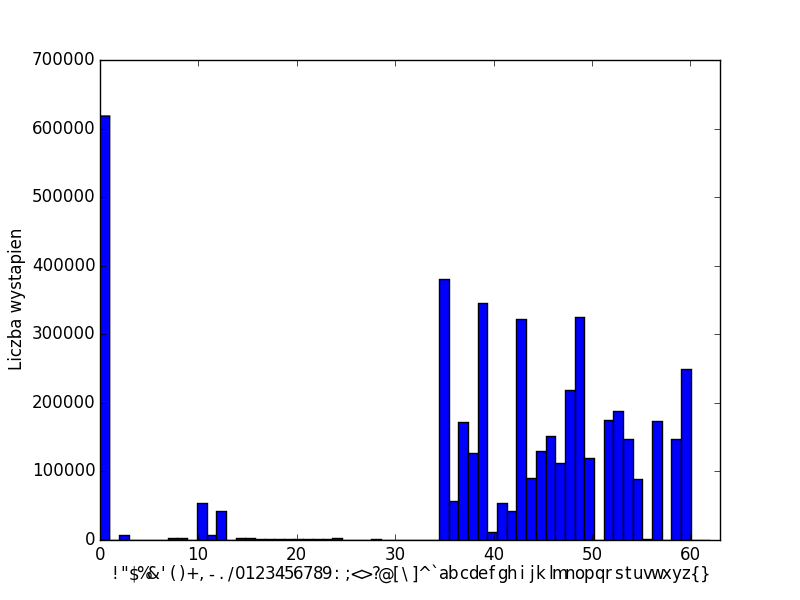
\includegraphics[width=0.5\textwidth]{pictures/char_letters_distribution.png}
    \caption{rozkład na danych dla modelu bazującego na znakach}
\end{figure}

\subsection{Podział na wyrazy}
Trochę statystyk z oryginalnych danych:
\begin{itemize}
    \item Liczba zdań: 45000
    \item Liczba słów: 100713
    \item Długość zdań: od 4 do 72 wyrazów, średnio: 14 wyrazów
\end{itemize}
\begin{figure}[!h]
    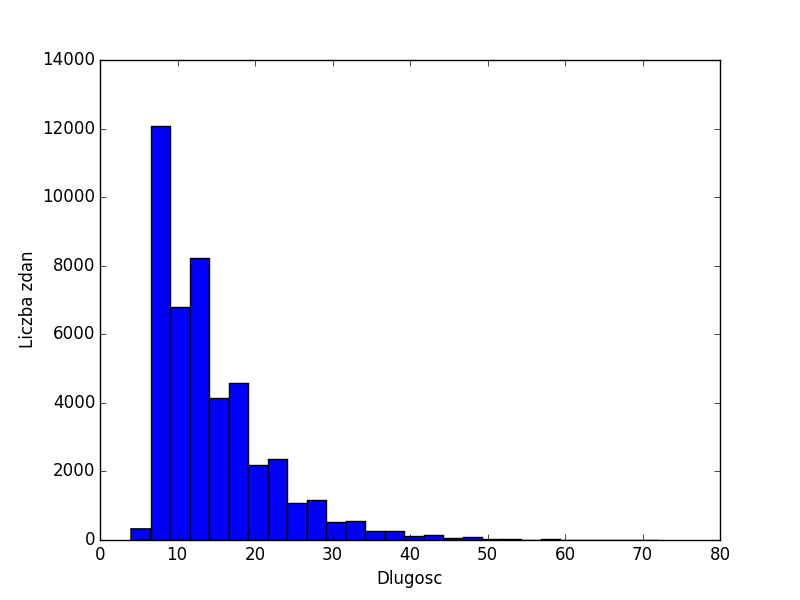
\includegraphics[width=0.5\textwidth]{pictures/word_length_distribution.png}
    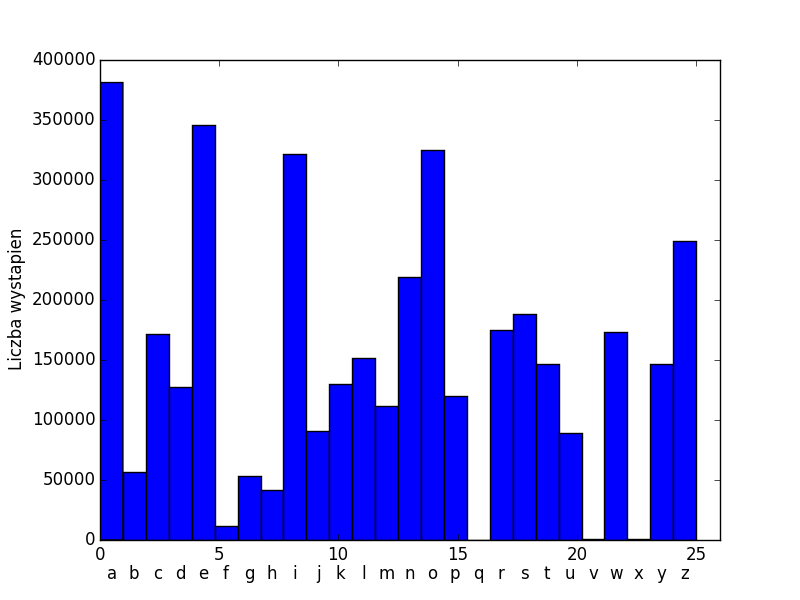
\includegraphics[width=0.5\textwidth]{pictures/word_letters_distribution.png}
    \caption{rozkład na danych dla modelu bazującego na słowach}
\end{figure}
\pagebreak
Niestety z racji tego że to trochę za dużo różnych słów musiałem je przefiltrować żeby dało się na tym w sensownej pamięci i czasie uczyć. Wybrałem poprostu najpopularniejsze wyrazy i zdania które je zawierają. \\
Trochę statystyk z przefiltrowanych danych:
\begin{itemize}
    \item Liczba zdań: 1931
    \item Liczba różnych wyrazów: 4028
    \item Długość zdań: od 4 do 34 wyrazów, średnio: 9 znaków
\end{itemize}
\begin{figure}[!h]
    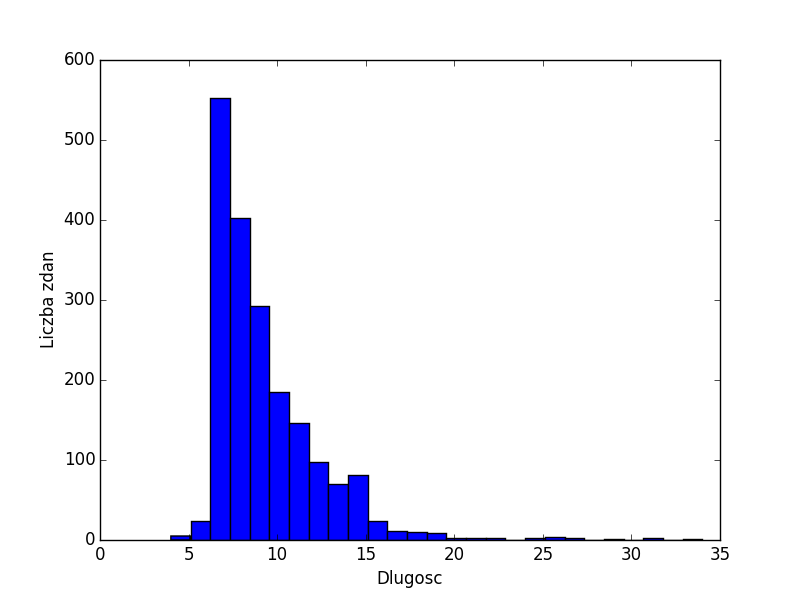
\includegraphics[width=0.5\textwidth]{pictures/word_filtered_length_distribution.png}
    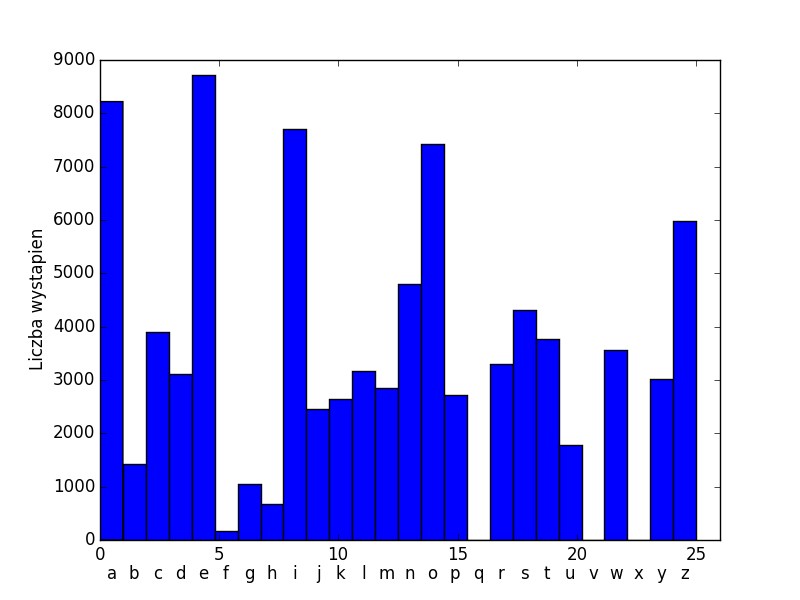
\includegraphics[width=0.5\textwidth]{pictures/word_filtered_letters_distribution.png}
    \caption{rozkład na przefiltrowanych danych dla modelu bazującego słowach}
\end{figure}

\section{Eksperymenty}
Na wstępie muszę zaznaczyć, że wykorzystanie Hesian-Free optimization pomimo tego że jest stabilniejsze to przez to że potrzeba na nie dużo więcej czasu(=mocy obliczeniowej) to w tym wypadku nie dało lepszych wyników od zwyczajnego SGD. \\
W związku z tym jedyne dane i wnioski są głównie na podstawie SGD, który przy dobrym doborze parametrów dawał szybko lepsze wyniki, i przy odrobinie szczęścia nie eksplodował. \\\\
Parametry do uczenia dobierałem robiąc przeszukiwanie binarne tak żeby znaleźć jak najlepszą szybkość uczenia i uniknąć eksplodowania gradientu. W praktyce jak miało się zepsuć to psuło się już gdzieś po maksymalnie kilkudziesięciu iteracjach na co na szczęście nie trzeba było czekać zbyt długo.
Wypróbowałem dwa podejścia reprezentowania tekstu w sieci - znak po znaku oraz podział na wyrazy.

\subsection{Znak po znaku}
W przypadku pierwszego jest on o tyle ciekawy że pozwala on na tworzenie zupełnie nowych wyrazów, ale jak się zaraz okaże sprawia też że generowane sekwencje dla osiągniętych przeze mnie wyników nie mają większego sensu poza danymi treningowymi.
Najlepszy wynik jaki udało mi się uzyskać to około 45\% poprawności na danych testowych, co sprawiło że niektóre nowe tworzone wyrazy wyglądały sensownie.

\begin{figure}[!h]
    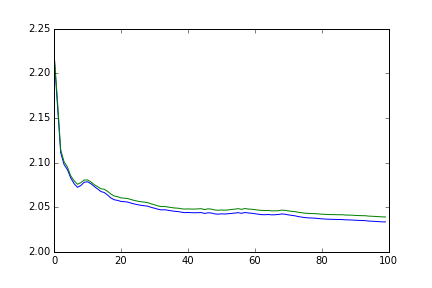
\includegraphics[width=0.5\textwidth]{pictures/char_progress-1.png}
    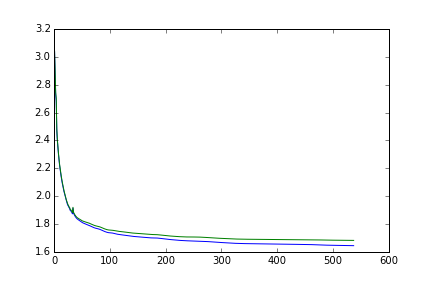
\includegraphics[width=0.5\textwidth]{pictures/char_progress-2.png}
    \caption{nauka znak po znaku do poprawności 30\% i 45\%}
\end{figure}

\begin{multicols}{2}
    Po kilkudziesięciu iteracjach: poprawność 30\% \\
    \begin{itemize}
        \item   to aoep solzi zdziysilzwo zie was palazy ppeatini p poeao zoe azi  \\
                kutki wypadku odczuwac bedzie juz zawsze  zlamana w kilku miejscas

        \item   tozcin ze o pozpo pie   zozzep e zwa     zwo polrrio podtowa a h p \\
                prawa, jaka ma do niej, musi wiec nalezec do gatunku pospolitych s

        \item   tere   po inze za   pooczami ptolzy  pola  z stwaepyasao apapiasz  \\
                talymi towarzyszami krystyny skarbek byli: wysoki blondyn z wlosas

        \item   teriezi  zo i ao  p po towznzi podezi pastazzneoe  ziszi p powiaow \\
                tanislaw gomulka: - gospodarka polska jest calkiem mocna i kontros
    \end{itemize}

    Przykładowe generowane sekwencje(pogrubione dane wejściowe): \\
    \textbf{caly swiat}hesa a\\
    \textbf{ala ma kota} a aa \\
    \textbf{nie mozna }a   a a

    \columnbreak
    Po tysiącu iteracji poprawność 48\% \\
    \begin{itemize}
        \item   tutei pykadku bdrzycaj tidzie mez nacsze snne ani w soeku miessco  \\
                kutki wypadku odczuwac bedzie juz zawsze  zlamana w kilku miejscas

        \item   trawa  nak  zagwoskaej  josimsyec ciwezy  do sarunku bowtrlitycz s \\
                prawa, jaka ma do niej, musi wiec nalezec do gatunku pospolitych s

        \item   aana   so arzyste i ooattyna iplrbu  zyl   systkienyondenglaniasy  \\
                talymi towarzyszami krystyny skarbek byli: wysoki blondyn z wlosas

        \item   aanislaw so e ki  " nlrcodarci polski pest pzlyoem mozny i control \\
                tanislaw gomulka: - gospodarka polska jest calkiem mocna i kontros
    \end{itemize}
    Przykładowe generowane sekwencje(pogrubione dane wejściowe): \\
    \textbf{caly swiat}zlesoni i wuclino worn.cona.  tokowacii ..lanni. lonui otalno \\
    \textbf{ala ma kota}le narkowali .. woko.c.  l nosc.wack. or..nacy ..nokaji ..r.. \\
    \textbf{nie mozna }a olatii  o i.waniu molasa.. .at..ni i wascinenki . losci  on
\end{multicols}

\subsection{Podział na wyrazy}
W tym przypadku nie wydzielałem zbioru testowego tylko starałem się jak najbardziej nauczyć sieć danych treningowych. Niestety z powodu większych danych (ok. 4000 wyrazów vs 63 litery) liczyło się trochę wolniej.

\begin{figure}[!h]
    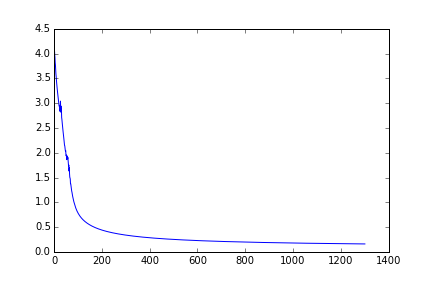
\includegraphics[width=0.5\textwidth]{pictures/word_progress.png}
    \caption{nauka po wyrazach do poprawności 70\%}
\end{figure}

\begin{multicols}{2}
    Po kilkuset iteracjach: poprawność 5\%\\
    \begin{itemize}
        \item   nie nie nie w w i i\\
                tak rzeczywiscie ci w niej do twarzy

        \item   nie nie nie w w i\\
                to teraz jest to u nas

        \item   nie nie \\
                wlasnie zaczal

        \item   nie nie nie jest w w i \\
                tego czasu nie ma umowy o prace
    \end{itemize}

    Przykładowe generowane sekwencje(pogrubione dane wejściowe): \\
    \textbf{takich} nie nie nie nie \\
    \textbf{nigdy} nie nie nie w w \\
    \textbf{miec troche wiecej} nie nie nie nie w i \\
    \textbf{uwazam ze} nie nie nie nie

    \columnbreak
    Po tysiącu iteracji: poprawność 30\%\\
    \begin{itemize}
        \item   bo pan jest wieku ty \\
                bo pan jest taki inny

        \item   tego robic nie ma jednak o mam \\
                tego czasu nie ma umowy o prace

        \item   dla kto z albo jest prawo drugie a kto prawo i raz \\
                wie kto z nas jest na pierwszym a kto na ostatnim miejscu

        \item   dla czego nie wiedzial obrony jest chce w \\
                po prostu nie wiedzial gdzie jest jego dom
    \end{itemize}

    Przykładowe generowane sekwencje(pogrubione dane wejściowe): \\
    \textbf{takich} dosc jak tez bylo wazne wiecej \\
    \textbf{nigdy} nie tak nie wie z kobieta razem wczesniej \\
    \textbf{miec troche wiecej} ze soba wszystko wie w nam gdyby kilka lat wszystko wie czym nam \\
    \textbf{uwazam ze} ze lat ma kazdy do mi kilka
\end{multicols}

\section{Wnioski}
Wykorzystanie RNN do generowania/analizy tekstu wydaję się być całkiem sensownym pomysłem.
Wydaje się że może to działać bardzo ładnie szczególnie jak zastosuje się optymalizacje HF, która niestety wymaga albo bardzo dużo czasu, albo większych mocy obliczeniowych.
W moim przypadku osiągnięte z SGD wyniki nie są może świetne, ale całkiem zadowalające.

\end{document}
